% Figure 8 of "Galashin's Conjecture 4.3 via a convex gradient": the resolved boundary and necklace for the window (3,5,6,7,9).
% Source of the figure, typeset in the paper's own fonts (T1, Latin Modern, 11pt) at the paper's text
% width (6.5in), so \includegraphics does not rescale it. Illustrates CLH-4; it adds no assertion.
% Every value drawn is read from these Lean output lines:
%   EX02 window(1-based)=[3, 5, 1, 2, 4] n=5 modulus=25 rank=3 coloops=[]
%   EX02 s_x (x=1..n)=[3, 4, 1, 5, 2]
%   EX02 exitPos(x=1..n)=[1, 6, 11, 16, 21]
%   EX02 entryPos(x=1..n, entry of strand into x)=[14, 19, 4, 24, 9]
%   EX02 crossEdges(paper labels)=[(1, 2), (2, 3), (2, 4), (3, 5), (4, 5), (5, 1), (5, 2)]
%   EX02 crossEdges with s_p=q (paper labels)=[(2, 4), (4, 5), (5, 2)]
%   EX02 necklace rows I_1..I_n=[[1, 2, 4], [2, 3, 4], [3, 4, 5], [1, 4, 5], [1, 2, 5]]
% Build: pdflatex <this file> && pdftocairo -svg <this file>.pdf <this file>.svg
\documentclass[11pt]{standalone}
\usepackage[T1]{fontenc}
\usepackage{lmodern}
\usepackage{amsmath,amssymb}
\usepackage{tikz}
\usetikzlibrary{arrows.meta,positioning,calc}

% the palette of the paper's other figures: blue solid for the first strand or arc, ochre dashed for the second
\definecolor{ink}{HTML}{233740}
\definecolor{muted}{HTML}{65757D}
\definecolor{pblue}{HTML}{0072B2}
\definecolor{qochre}{HTML}{B87827}

\tikzset{
  base/.style={draw=muted, line width=0.5pt},
  exit/.style={circle, draw=ink, fill=white, line width=0.6pt, inner sep=0pt, minimum size=4.6pt},
  entry/.style={circle, draw=ink, fill=ink, line width=0.6pt, inner sep=0pt, minimum size=4.6pt},
  exitP/.style={exit, draw=pblue}, entryP/.style={entry, draw=pblue, fill=pblue},
  exitQ/.style={exit, draw=qochre}, entryQ/.style={entry, draw=qochre, fill=qochre},
  strandP/.style={pblue, line width=1.1pt, -{Stealth[length=5pt,width=4.2pt]}, shorten >=2.4pt},
  strandQ/.style={qochre, line width=1.1pt, dash pattern=on 4pt off 1.6pt, -{Stealth[length=5pt,width=4.2pt]}, shorten >=2.4pt},
  lab/.style={font=\footnotesize, inner sep=1.2pt, text=ink},
  labm/.style={font=\small, inner sep=1.2pt, text=ink},
  labP/.style={font=\small, inner sep=1.2pt, text=pblue},
  labQ/.style={font=\small, inner sep=1.2pt, text=qochre},
  muted text/.style={text=muted},
  ttl/.style={font=\small, text=ink, inner sep=0pt},
  negE/.style={font=\small, text=pblue, inner sep=0pt},
  posE/.style={font=\small, text=qochre, inner sep=0pt},
  zeroE/.style={font=\small, text=ink, inner sep=0pt},
  idx/.style={font=\footnotesize, text=muted, inner sep=0pt},
}

\begin{document}
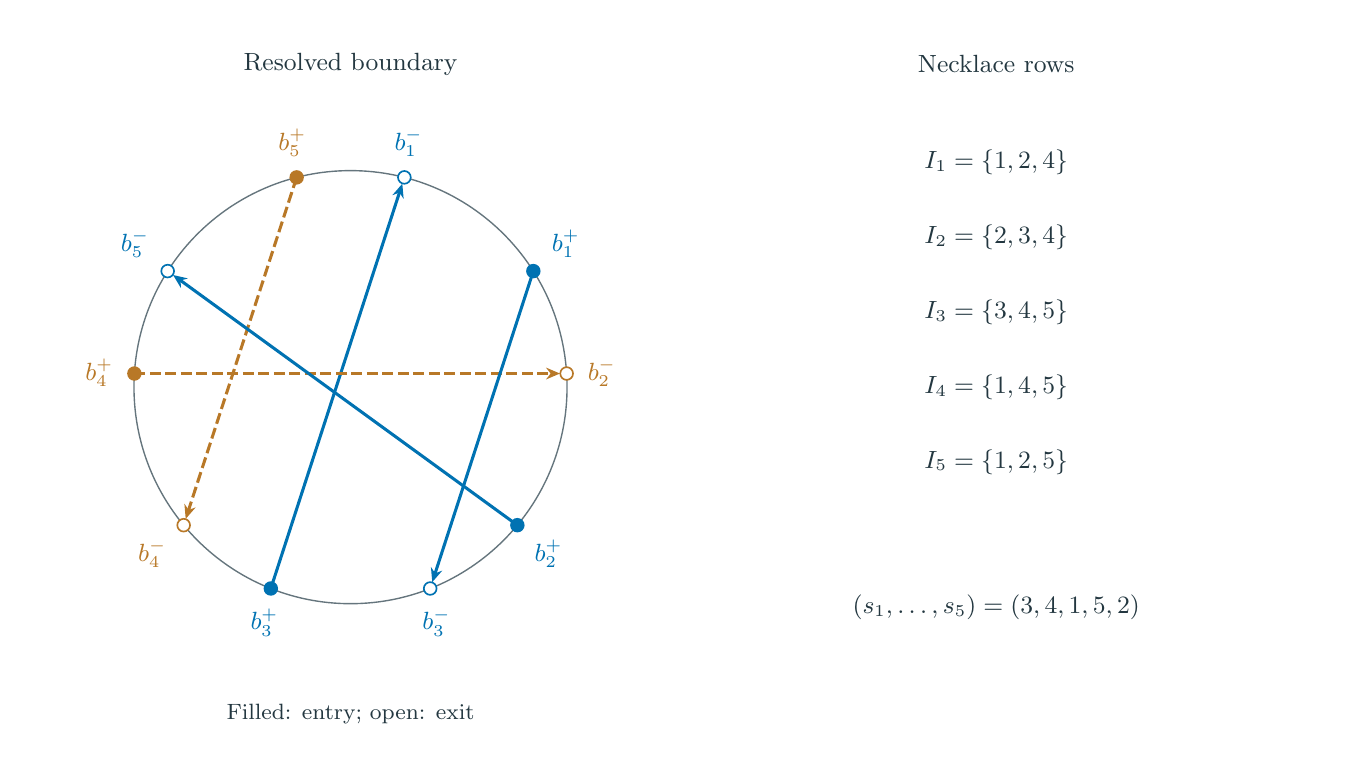
\begin{tikzpicture}[x=1cm,y=1cm]
\useasboundingbox (-0.25000,-8.76527) rectangle (16.26000,0.36527);
\node[ttl] at (3.850,-0.100) {Resolved boundary}; %t title0
\draw[base] (3.850,-4.200) circle (2.750); %o 0 25
\draw[strandP] (2.838,-6.757) -- (4.534,-1.536); %s 1 14 1
\node[exitP] at (4.534,-1.536) {}; %p exit1 1
\node[labP, anchor=south] at (4.589,-1.323) {$b^{-}_{1}$}; %t exit1
\node[entryP] at (2.838,-6.757) {}; %p entry1 14
\node[labP, anchor=north] at (2.757,-6.961) {$b^{+}_{3}$}; %t entry1
\draw[strandQ] (1.105,-4.027) -- (6.595,-4.027); %s 2 19 6
\node[exitQ] at (6.595,-4.027) {}; %p exit2 6
\node[labQ, anchor=west] at (6.814,-4.014) {$b^{-}_{2}$}; %t exit2
\node[entryQ] at (1.105,-4.027) {}; %p entry2 19
\node[labQ, anchor=east] at (0.886,-4.014) {$b^{+}_{4}$}; %t entry2
\draw[strandP] (6.172,-2.726) -- (4.862,-6.757); %s 3 4 11
\node[exitP] at (4.862,-6.757) {}; %p exit3 11
\node[labP, anchor=north] at (4.943,-6.961) {$b^{-}_{3}$}; %t exit3
\node[entryP] at (6.172,-2.726) {}; %p entry3 4
\node[labP, anchor=south west] at (6.358,-2.609) {$b^{+}_{1}$}; %t entry3
\draw[strandQ] (3.166,-1.536) -- (1.731,-5.953); %s 4 24 16
\node[exitQ] at (1.731,-5.953) {}; %p exit4 16
\node[labQ, anchor=north east] at (1.562,-6.093) {$b^{-}_{4}$}; %t exit4
\node[entryQ] at (3.166,-1.536) {}; %p entry4 24
\node[labQ, anchor=south] at (3.111,-1.323) {$b^{+}_{5}$}; %t entry4
\draw[strandP] (5.969,-5.953) -- (1.528,-2.726); %s 5 9 21
\node[exitP] at (1.528,-2.726) {}; %p exit5 21
\node[labP, anchor=south east] at (1.342,-2.609) {$b^{-}_{5}$}; %t exit5
\node[entryP] at (5.969,-5.953) {}; %p entry5 9
\node[labP, anchor=north west] at (6.138,-6.093) {$b^{+}_{2}$}; %t entry5
\node[lab] at (3.850,-8.350) {Filled: entry; open: exit}; %t legend
\node[ttl] at (12.050,-0.100) {Necklace rows}; %t title1
\node[labm] at (12.050,-1.350) {$I_{1}=\{1,2,4\}$}; %t necklace0
\node[labm] at (12.050,-2.300) {$I_{2}=\{2,3,4\}$}; %t necklace1
\node[labm] at (12.050,-3.250) {$I_{3}=\{3,4,5\}$}; %t necklace2
\node[labm] at (12.050,-4.200) {$I_{4}=\{1,4,5\}$}; %t necklace3
\node[labm] at (12.050,-5.150) {$I_{5}=\{1,2,5\}$}; %t necklace4
\node[labm] at (12.050,-7.000) {$(s_{1},\dots,s_{5})=(3,4,1,5,2)$}; %t sx
\end{tikzpicture}
\end{document}
